
\documentclass[]{exam}
\title{\centering CS684 Embedded Systems(Software) , Project Report \newline \centering Self Orienting Smart Chair}

\usepackage{amsmath}
\usepackage{graphicx}
\usepackage{subcaption}
\usepackage{color}
\usepackage{epstopdf}
\usepackage{graphics}

\author{Patil Akhilesh Subhash (173079005), Supriya Asutkar(174360005),Rahul Pari(173100041)}



\begin{document}

\maketitle

\hrule

\tableofcontents
\fbox{git Repository for all codes :https://github.com/akhileshiitb/CS684-2018 }

\newpage 
\section{\color{red} Introduction }
\paragraph{•}
We often find in offices , or in labs , Chairs are not oriented properly . Sometimes we become little lazy and do not place chairs in proper positions. The aim of this project is to design a prototype for self orienting smart chair which can localize itself and navigate to the desired position. The future outcome of this project is like consider a situation where all chairs are randomly oriented inside a room. When we give command all chairs should get automatically oriented and nevigate to their default positions.

Figure \ref{intro}  shows the scene from hostel 1 , where at night chairs were randomly oriented and it looks messy. Our motivation for this project was from here. These chair should  be smart enough to orient and organize properly as shown in right picture. For that we need to have mechanism to localize the chairs and then move accordinly to the destinations to organize them properly. 
\begin{figure}[h!]


 \centering
 
  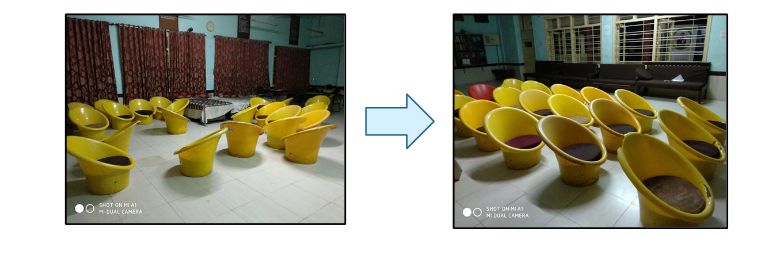
\includegraphics[scale=0.5]{intro.png}
  \caption{Problem Statement }
  \label{intro}
  \end{figure}
    

\section{\color{red} Problem Statement }
\paragraph{•}
In this project our problem statement is to make prototype of such self orienting chair. We take firebird V robot as a chair . We will put robot at any place in coverage area i.e arena in any random orientation. Our aim is to detect its position and orientation and accordingly reorient robot in proper position and navigate it till its original position. 
\paragraph{•}
 So in this prototype we are orienting and organizing firebird robots. We will take 2 robots at the same time and they should reach at two differnt predefined destination positions. There should not be any collison between them. Here We are listing some of the challenges thay may be faced doing it. 
 \begin{itemize}
 \item Setup was a big challenge. The area taken by camera, its resolution so that it can detect arUco from maximum possible height. The camera was fitted on a L shaped structure made of pipes of height approximately 2.7 m. 
\item Detection of marker using ArUco was an another challenge. The complexity increases when multiple markers were used. Accurate mapping of arUco position from real world to server computer was a difficult task.  
\item  Then comes, Communication between firebird robot and server computer. Multiple arUco, and firebird with single camera and server computer made it a tough.
\item Xbee – Defining the role of each module pair to a specified ID and robot. 
\item  Calculation of path for navigation involved mapping of real and virtual coordinates. Finding how inertia of firebird will play with rotation, moving forward, acceleration and braking in order to make necessary changes in the program for desired functioning of robot.
\end{itemize}  

\section{\color{red} Requirements }
Folowing are the requirement of this prototype design 
\begin{itemize}
\item \textbf{Hardware :} 
\begin{itemize}
\item \textbf{Firebird V} : This will be our prototypr chair . We will place 2 firebird V robots in the arena with aruco marker placed on the top of it. these robots has to nevigate upto destination. 
\item \textbf{Camera }: USB camera is required to capture the arena feed and send to laptop/computer fot image processing(i.e detecting aruco markers)
\item \textbf{Xigbee Module} : Zigbee modules are user for communication betwee server/computer and firebird robot. 
\item \textbf{Zigbee Explorer} : It is used to connect Xbee module to computer via USB port 

\end{itemize}

\item \textbf{Software :} 
\begin{itemize}
\item \textbf{Embedded C} : This is programming language we use to program ATMEGA2560 controller of firebird . 
\item \textbf{OpenCv and Aruco library} : These libraries are used to implement image processing in our project. 
\item \textbf{Python :} Entire aruco detection and decision making code is written in python using aruco and opencv libraries.  
\item \textbf{XCTU : } This software is from DigiKey is used for configuring Xbee modules. 
\item \textbf{Code Blocks IDE :} Required IDE for embedded C program development 
\item \textbf{AVRdude :} To burn Hex files on firebird 
\end{itemize}
\end{itemize}
\begin{figure}[h!]


 \centering
 
  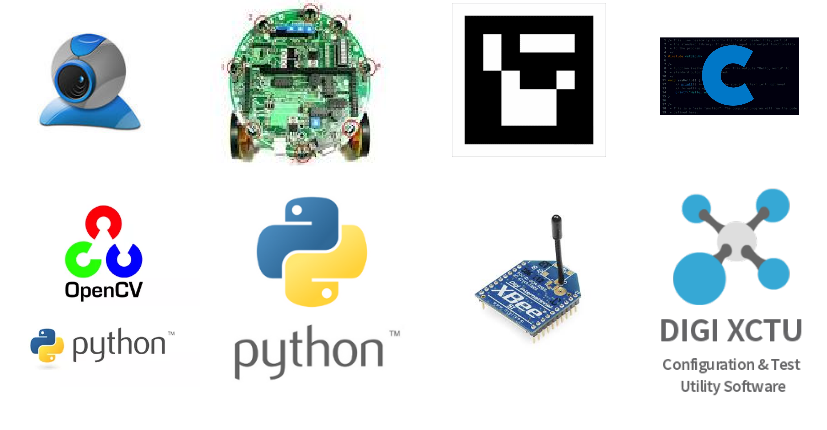
\includegraphics[scale=0.6]{req.png}
  
  \label{req}
  \end{figure}


\newpage
\section{\color{red} System Design }
\paragraph{•}
\begin{figure}[h!]


 \centering
 
  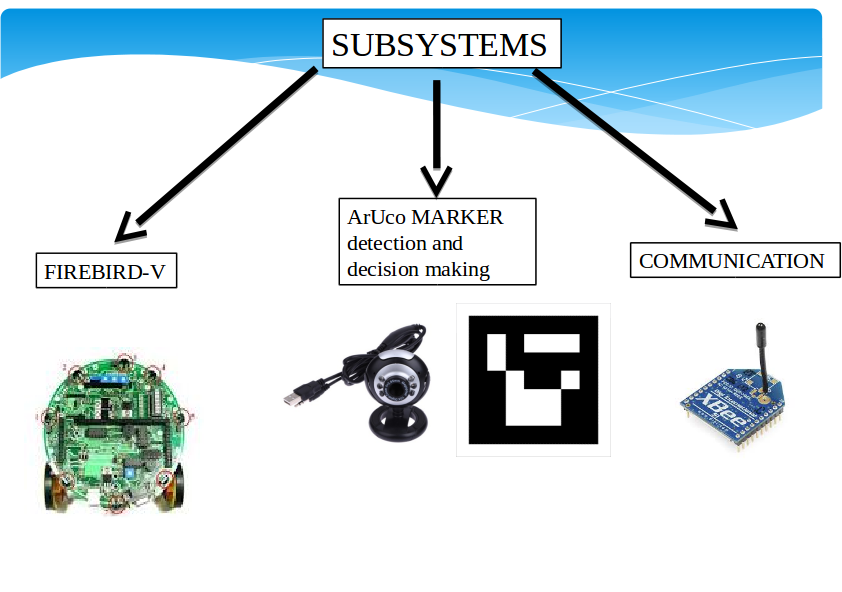
\includegraphics[scale=0.4]{system.png}
  \caption{the System }
  \label{system}
  \end{figure}
For better understanding of the system , we present our system in three parts as shown by the figure \ref{system},  Firebird navigation part , aruco marker detection using image processinga and communciation between computer and firebird. 
Figure \ref{block_diagram} show the overall block diagram of our system. We will note down some of the important points of our systems with reference to the block diagram shown in Figure \ref{block_diagram} 

\begin{itemize}
\item Web camera is used to take live video from arena. It will be fixed on the roof or using stand at some distance above the arena. It will take live video and feed it to laptop/server. Each firebird robot will have predefined aruco code printed on it.
\item Job of the server is to get the video feed from camera and process it . Then using image processing , server determines aruco markers inside the arena and hence the positions of firebird robots. It uses aruco and opencv library to calculate positions and ids  of aruco markers. Another job of server is to determine the position and guide firebird to navigate. 
\item When we get the positions of firebird we decide what will be the trajectory of the firebird using python code and this decisions are conved to the firebird via Zigbee connectivity. 
\item once decisions regarding trajectory are received by the firebird. Firebird moves according to messages gicen by the server via Zigbee connectivity. 
\item Note that there is Continuous feedback taken from firebirds changing positions. i.e when firebird moves each time images are taken and updated values of positions are processed in server and trajectory decisions are updated and conveyed to firebird again and this goes on continuously till firebird reaches at its destination. 
\item in case of 2 firebird. We have desinged our system such that in first slot 1st firebird moves and reach the destination while 2nd firebord is stationary. and In second slot 2nd firebird moves while 1st is stationary. This is done to avaoid collision between two. 
\end{itemize} 

\begin{figure}[h!]


 \centering
 
  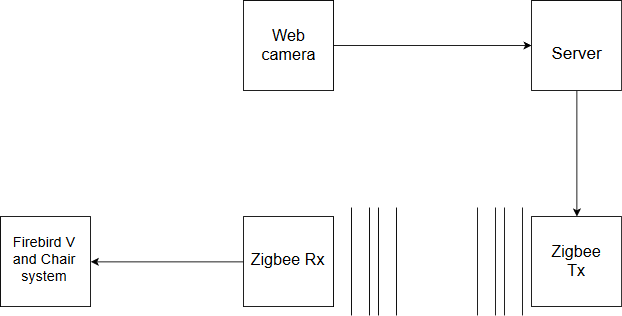
\includegraphics[scale=0.65]{block_diagram.png}
  \caption{Block Diagram of the System }
  \label{block_diagram}
  \end{figure}
  
  


\subsection{\color{red} Aruco Marker detection and decision making}
Figure \ref{algo} shows the algorithum used for our sytem to detect positions and make decisions. We will explain it step by step 
\begin{itemize}
\item First we read video from camera and take a scanpshot.We use openCV and aruco library for programming in python. 
\item Then we detect aruco markers in the image i.e positions of firebird.
\item Then we have predefined positions of destination. We compare this with current location of firebird and send necessary messages to firebird which help firebird to navigate. 
\item if destination is reached or location of firebird is in some neighbourhood of destination defined by threshold then we send stop command to firebird else we repeat the precess of navigation. 
\end{itemize}

\begin{figure}[h!]


 \centering
 
  
\includegraphics[scale=0.35]{out.png}
  \caption{Aruco marker  }
  \label{out}
  \end{figure}
\begin{figure}[h!]

 \centering
 
  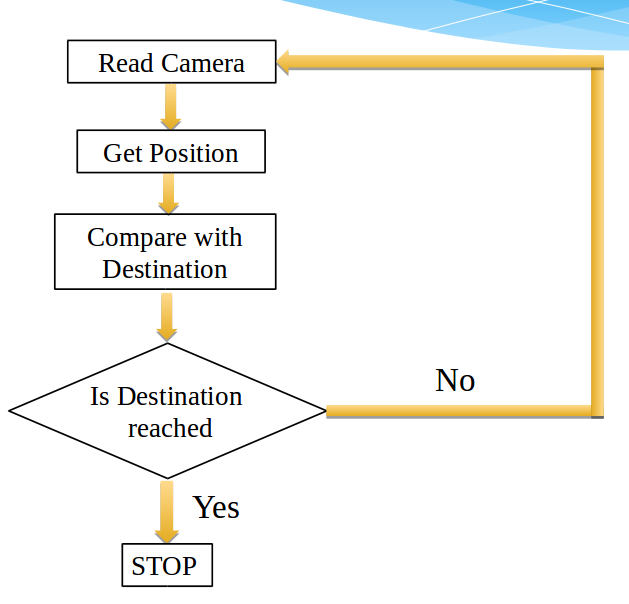
\includegraphics[scale=0.6]{algo.png}
  \caption{System flow chart  }
  \label{algo}
  \end{figure}
  \newpage
  \subsection{\color{red} Firebird Programming }
  
  \paragraph{•}
  
  
  
  
  \begin{itemize}
  \item Position encoders : We use firebirds position encoders / rotatory encoders to get the feedback of how much distance and how much angle firebird is moving. So that we can move in steps of 10mm and can rotate in steps of 5 degrees to wait for next decision message form server. 
  
  \item Motor contel : This section deals with controlling movement of wheels of firebord.
  
  \item UART Communication :  messages are received using UART communication , hence firebord is programmed to receive data coming at UART0 pin of ATMEGA2560. Code can be found in code section of the submission.We get navigation decisions from server via Zigbee. Firebird reads it using UART receiver and decodes these messages to navigate. Firebird is controlled using just 4 messages sent from server. These are listed bwlow: 
  \begin{itemize}
  \item A  : Rotate Right by 5 degree 
  \item R : Turn 90 degree Right 
  \item L : Turn 90 degree Left 
  \item F : Move Forward 10mm 
  \end{itemize} 
  \end{itemize}
  
  
\subsection{\color{red} Communication}
\begin{itemize}
\item This module consists of communication link between Server and firebird to convey messages regarding navigation. We use Zignee S2 modules. 
\item We configure both Zigbee modules for operating in C band. And both tranmisste and receiver pair should be on same network defined by PAN(Personal Area Network ) ID. 
\item Zigbee module on server side is configured as a Coordinator and Zigbee module installed on firebird is configured as a end device. 
\item We use XCTU software from digiKey to Configure the Zigbees. 
\item At the coordinator we put destination address of end device (i.e firebird Xbee) and vice versa. This way two Xbees are alble to so communication. 
\item While sending messages from server we send characters using python commands serial.send('/dev/ttyUSB') where /dev/ttyUSB is out serial port of server.   
\end{itemize}

Figure \ref{xctu} shows typical window for XCTU software where we can configure our xbees i.e we can set PAN ID , channel , destination addredd , Mode and allother related parameters. 
\begin{figure}[h!]


 \centering
 
  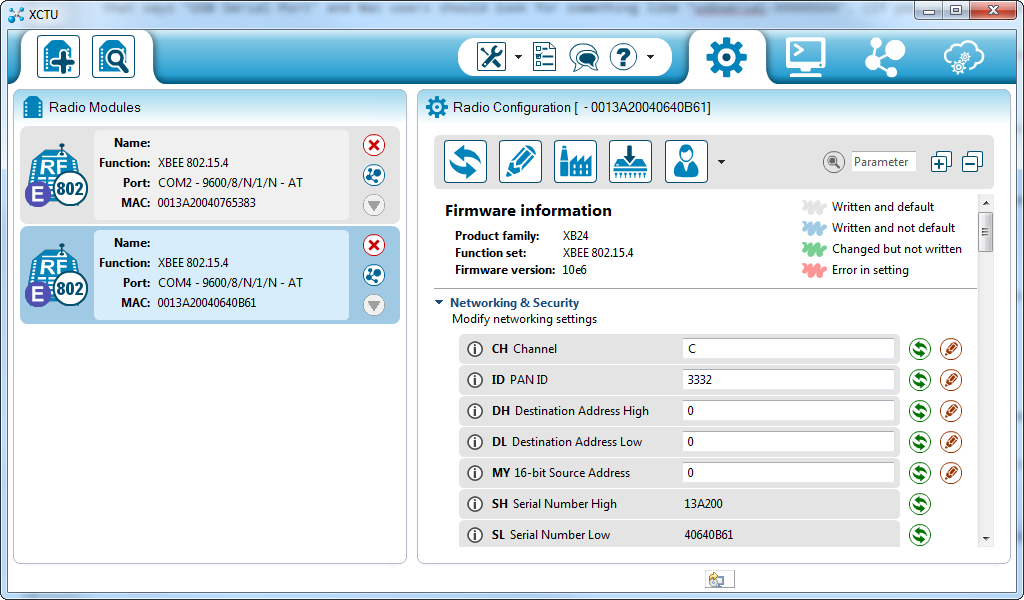
\includegraphics[scale=0.6]{xctu.png}
  \caption{XCTU software from DigiKey }
  \label{xctu}
  \end{figure}
  \newpage
\section{\color{red} Working of System and Test results }

\paragraph{•}
When position of firbird is detected by the camera.We decide weather firebird is on left or right of the desination. Then first firebird gets oriented to refernce direction by rotating according to messages sent by server . Then if firebird is on left hand side then it first moves along x axis then taked 90 degree left turn and moves along y direction till it reaches close to the destination. Similar actions are taken when firebird is at right hand side. These movements of firebird are according to decision messages sent from server after image processing and decision algoritum. Following are the results 

\begin{itemize}
\item Figure \ref{webcam} shows the camera setup . Camera is mounted on the L shaped stand as shown this this figure. 
\item Figure \ref{init} shows the initial positions for both firebird 1 and 2 and their destinations.
\item Figure \ref{detected} shows feed from camera and detected the aruco markers on it. 
\item Figure \ref{dest} shows two firebird robots reached their destinations.
\end{itemize}



  \begin{figure}[h!]
 \centering 
  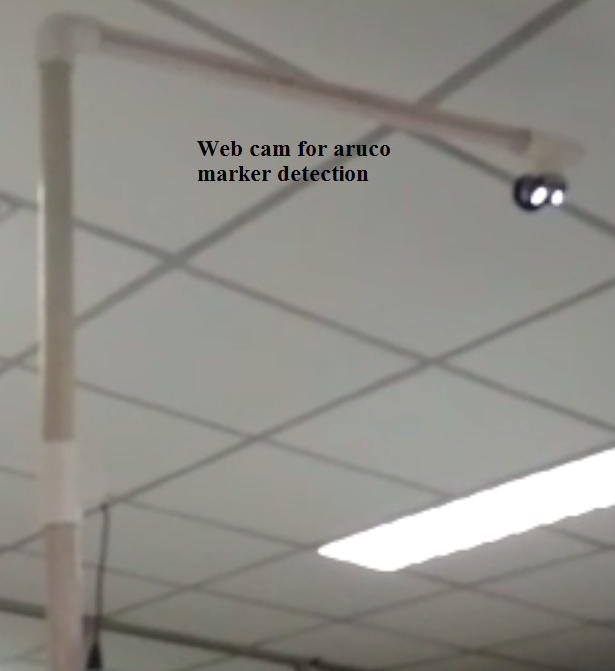
\includegraphics[scale=0.5]{webcam.png}
  \caption{webcam setup }
  \label{webcam}
  
  
  \end{figure}
  
\begin{figure}[h!]
 \centering 
  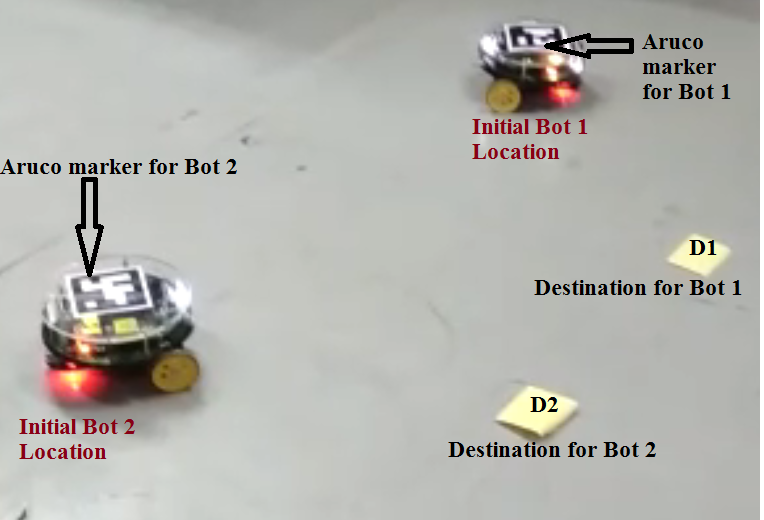
\includegraphics[scale=0.5]{init.png}
  \caption{Initial position }
  \label{init}
  \end{figure}
  
  
   \begin{figure}[h!]
 \centering 
  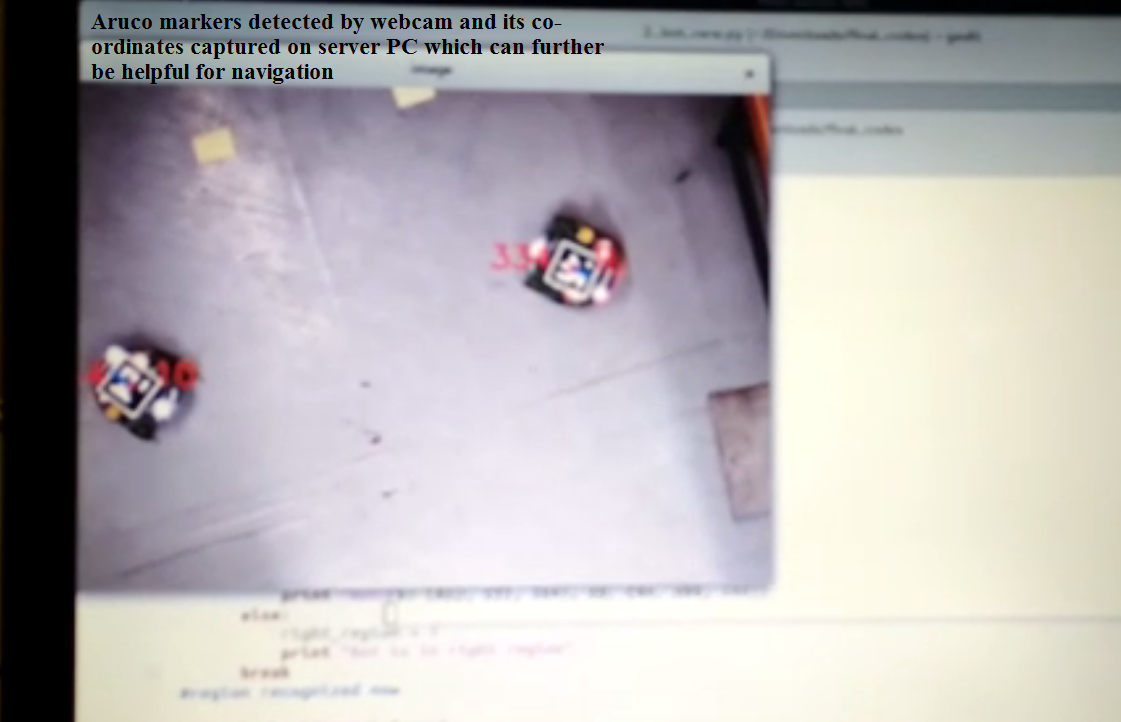
\includegraphics[scale=0.38]{detected.png}
  \caption{Detection of the marker  }
  \label{detected}
  \end{figure}
  
  
  \begin{figure}[h!]
 \centering 
  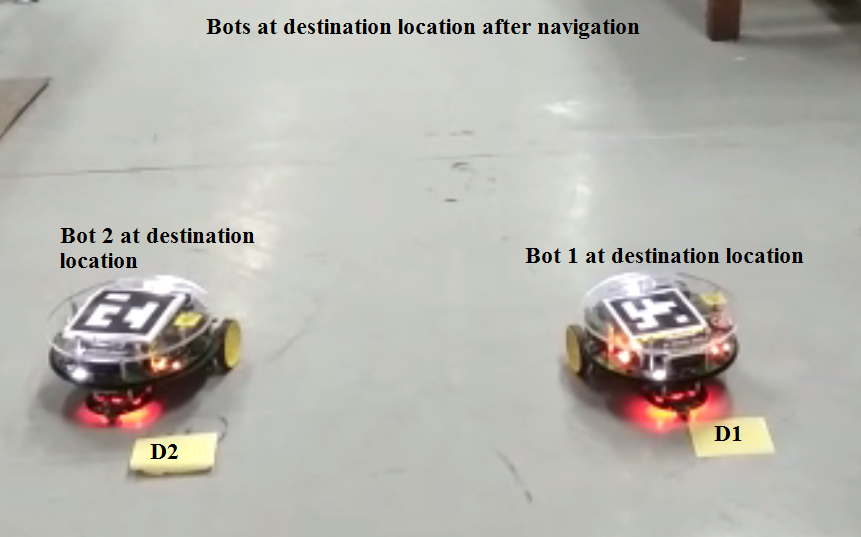
\includegraphics[scale=0.5]{dest.png}
  \caption{Destination reached }
  \label{dest}
  \end{figure}
  


\section{\color{red} Discussion of The System  }

\begin{itemize}
\item \textbf{Camera setup :} WE use L shaped stand to place a web camera to capture arena video. Initally we faced some problems while calibrating and focus the camera. The coverage are obtained from the camera was less. Thus we need to use wide angle camera to get expanded feed in the future. 
\item \textbf{Accuracy : } The accuray of the system depends on calibration of the camera. The distances that we get from image processing and actual physical distance we have to travel are differnt , hece we have to map virtual distance with actual distance and send that values to firebird. Hence that mapping or conversion should be accurate. And our accuray depends on this. Also accuray depends on sensitivity of position encoders on firebird also. Sometimes it may move little more or less than expected , in these cases there may be some accuracy errors. 
\item \textbf{Aruco detection : } Sometimes due to unclear images aruco markers are not detected , our system should be able to take care in this situation also.
\item Navigation method that we implemented here is not unique , one may come up with any method. Like from initial position first oreint in the direction of destination and then move straight twowards the destination. Or any other method can also be there. 
\end{itemize}

\section{\color{red} Future Work  }
\paragraph{•}
In this project we checked the possibility of implementing self orienting chairs using firebird robot and image processing. In Future we can go ahed and try to implement it on actual chairs. In this case we have to make a wheel system which gets fits to the existing chair to give it loccomotion according to messages sent by server. WE need high torque and omnidirectional wheels for making such system and Any conteoller like ATMEGA or PIC can be used to communication with server and moving accordingly  to reach the destination. We can also plan to use wide angle camera to cover larger area. We can go ahead and implement mechanism to avoid collision when more than one chairs are moving simultaneously. 
\section{\color{red} Conclusions }

\begin{itemize}
\item We were able to generate aruco markers and detect it . It is possible to generate and detect aruco maekers using webcamera and opencv libraries. 
\item aruco markers can be used to detect the position of the object as well as it can be used to detect the orinetation of the object. 
\item position encodes can be used to move robot by accurate distances. 
\item Communication between server computer and conteoller can be established using Xbee wireless connectivity and UART serial communication. 
\item In this experiment two firebird robot , initially placed in any random orientation and place in the arena , reached destination with some tolerable accuracy. This accuracy can be improved in the future by using more accurate position sensors and advanced path planning algoritum. Also arena feed can be improved using wide angle camera. 
\item This prototype worked well in indoor case with good lightning conditions.Firebird robot can be replaced with actual chair to get this project to next level. 
\end{itemize}
\section{\color{red} References  }
\begin{thebibliography}{9}
\bibitem{latexcompanion} 

\textit{https://www.sparkfun.com/products/11215description-tab}

 
\bibitem{einstein} 

\textit{http://www.nex-robotics.com/products/humanoid-robot/fire-bird-v-atmega2560-robotic-research-platform.html}

 
\bibitem{knuthwebsite} 
Visual localization of mobile robot using artificial markers
\texttt{Andrej Babineca
, Ladislav Jurišicaa
, Peter Hubinskýa
, František DuchoĖa}

\bibitem{einstein}
Some of the videos from Youtube.com 
\end{thebibliography}

\hrulefill

\end{document}